\paragraph{V4 - Rust}

Die V4 Variante wurde ebenfalls in Rust entwickelt, aber von Grund auf neu aufgebaut. Die Architektur wurde komplett überarbeitet und stark vereinfacht. Die \Gls{statemachine} wurde verworfen und die ganze Applikation basiert auf dem Datenbank \Gls{listener}. Der Listener wurde mithilfe Funktionalität der \texttt{firestore\_rs} Softwarebilbiothek Implementiert.

\subparagraph{Projektstruktur}

Das Projekt wurde mit \texttt{cargo new} erstellt, deshalb ist die Projektstruktur wie folgt:

\dirtree{%
  .1 tower\_controller\_v4.
  .2 src.
  .3 bin.
  .3 entities.
}

\begin{itemize}
  \item \textbf{\texttt{tower\_controller\_v4}} Root Verzeichnis des Projekts, hier befinden sich alle    Konfigurationsdateien (Cargo.toml, Cargo.lock, .gitignore, etc\ldots{}).
  \item \textbf{\texttt{src}} Hier befinden sich alle Quellcode Dateien.
  \item \textbf{\texttt{bin}} Hier befinden sich alle Quellcode Dateien, die Ausgeführt werden können.
  \item \textbf{\texttt{entities}} Hier befinden sich die Serialisierbaren Datenstrukturen (Entities), die den Dokumenten in der Datenbank entsprechen.
\end{itemize}

\subparagraph{Programmablauf}
\begin{enumerate}
  \item Der Turm Controller wird mittels der \texttt{main} Funktion gestartet.
  \item Umgebungsvariablen werden geladen.
  \item Datenbank Interface wird erstellt (\texttt{TowerDatabase::new}).
  \item Turm Datenstruktur wird erstellt und mit den Daten aus der Datenbank initialisiert (\texttt{Tower::new}).
  \item Assignment Scheduler wird erstellt (\texttt{AssignmentScheduler::new}).
  \item Der Scheduler wird gestartet (\texttt{AssignmentScheduler::start}) und der main \Gls{thread} wird in einen \Gls{sleep} Modus versetzt.
  \item Das Programm wartet nun auf Änderungen in der Datenbank.
\end{enumerate}

\begin{figure}[ht]
  \centering
  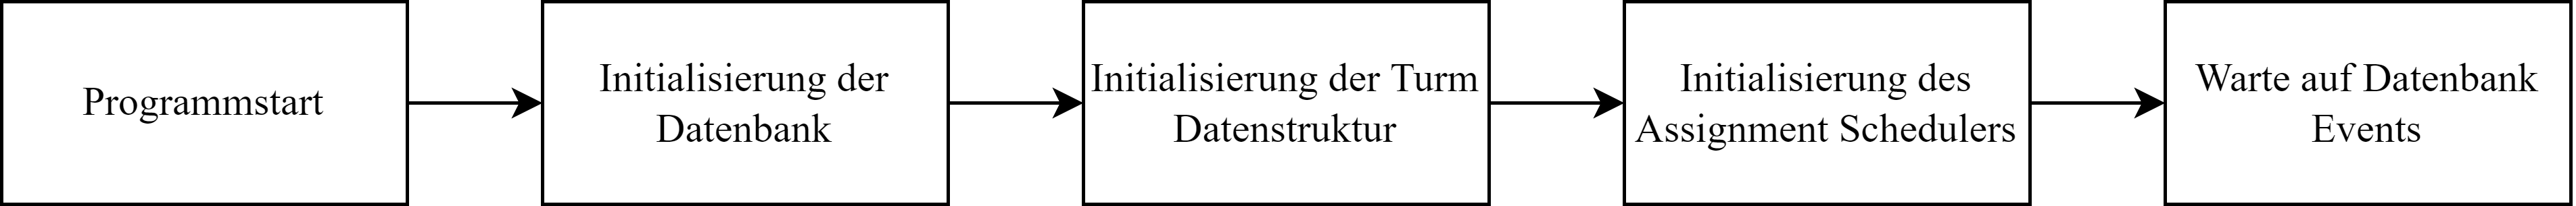
\includegraphics[width=1\textwidth]{images/tower_controller_v4_init.png}
  \caption{Intialisierung des Turm Controllers}
  \label{fig:tower_controller_v4_init}
\end{figure}

\subparagraph{{TowerDatabase}}

\texttt{TowerDatabase} kümmert sich um die Kommunikation mit der Datenbank. Es ist ein \Gls{wrapper} für die Datenbankverbindung der \texttt{firestore\_rs} Softwarebilbiothek. Es soll die interaktion mit der Datenbank vereinfachen und die möglichkeit von Fehlern minimieren.

\begin{minted}{rust}
struct TowerDatabase {
    db: FirestoreDb,
    tower_id: String,
    project_id: String,

    // This might be a bit overkill
    async fn new(project_id: &str, tower_id: &str) -> Result<Self, ControllerError>;

    async fn has_subscription(&self, m: &FirestoreJob) -> Result<bool, ControllerError>;

    async fn set_error(&self, a_id: &str, err: ControllerError) -> Result<(), ControllerError>;

    async fn set_confirm(&self, a_id: &str, con: ConfirmType) -> Result<(), ControllerError>;

    async fn set_slot(&self, a_id: &str, slot: &Vec<u32>) -> Result<(), ControllerError>;

    async fn create_listener(&self) -> Result<FirestoreListener<FirestoreDb, HashMapTokenStorage>, ControllerError>;

    async fn get_tower(&self) -> Result<(String, Vec<u32>, HashMap<Vec<u32>, Slot>), ControllerError>;

    async fn create_boxes(&self, dimensions: &Vec<u32>) -> Result<Vec<FirestoreBox>, ControllerError>;

    async fn delete_all_boxes(&self) -> Result<(), ControllerError>;

    async fn new_rental(&self, user_id: &str, box_location: &Vec<u32>) -> Result<String, ControllerError>;

    async fn finish_rental(&self, user_id: &str, box_location: &Vec<u32>) -> Result<(), ControllerError>;
}
\end{minted}

Felder:
\begin{itemize}
  \item \textbf{\texttt{db}}: Datenbankverbindung.
  \item \textbf{\texttt{tower\_id}}: ID des Turms.
  \item \textbf{\texttt{project\_id}}: ID des Projekts.
\end{itemize}

Methoden:
\begin{itemize}
  \item \textbf{\texttt{new}}: Erstellt eine neue Instanz von \texttt{TowerDatabase}.
  \item \textbf{\texttt{has\_subscription}}: Prüft ob ein nutzer eine Abonnement hat.
  \item \textbf{\texttt{set\_error}}: Setzt einen Fehlerstatus eines Assignments.
  \item \textbf{\texttt{set\_confirm}}: Setzt einen Bestätigungsstatus eines Assignments.
  \item \textbf{\texttt{set\_slot}}: Setzt einen Slot eines Assignments.
  \item \textbf{\texttt{create\_listener}}: Erstellt einen Listener, welcher auf Änderungen in der \texttt{jobs} Collection wartet.
  \item \textbf{\texttt{get\_tower}}: Lädt die Daten des Turms aus der Datenbank (Wichtigt für die Initialisierung des Turms).
  \item \textbf{\texttt{create\_boxes}}: Erstellt fehlende Boxen in der Datenbank anhand des Layout Felds.
  \item \textbf{\texttt{new\_rental}}: Erstellt einen neuen Mietvorgang in der Datenbank (users > rentals).
  \item \textbf{\texttt{finish\_rental}}: Beendet einen Mietvorgang in der Datenbank.
\end{itemize}


\subparagraph{Tower}

\texttt{Tower} ist die Datenstruktur des Turms. Sie enthält alle Informationen über den Turm und die Boxen. Sie wird von der \texttt{AssignmentScheduler} Klasse verwendet, um die Boxen zu verwalten. Tower enthält zusätzlich Methoden um die Datenstruktur zu verwalten.


\begin{minted}{rust}
struct Tower {
    id: String,
    slots: HashMap<Vec<u32>, Slot>,
    layout: Vec<u32>,
    db: Arc<TowerDatabase>,

    async fn new(db: Arc<TowerDatabase>) -> Result<Self, ControllerError>;

    fn find_free_slot(&self, slot_type: BoxType) -> Result<Vec<u32>, ControllerError>;

    async fn store_object(&mut self, slot: &Vec<u32>, user: &str) -> Result<(), ControllerError>;

    async fn retrieve_object(&mut self, slot: &Vec<u32>, user: &str) -> Result<(), ControllerError>;

    fn slot_exists(&self, slot: &Vec<u32>) -> Result<bool, ControllerError>;

    fn slot_rented_by_user(&self, slot_location: &Vec<u32>, user_id: &str) -> Result<bool, ControllerError>;

    async fn rent_box(&mut self, user_id: &str, slot_location: &Vec<u32>) -> Result<(), ControllerError>;

    async fn unrent_box(&mut self, user_id: &str, slot_location: &Vec<u32>) -> Result<(), ControllerError>;
}
\end{minted}

Felder:
\begin{itemize}
  \item \textbf{\texttt{id}}: ID des Turms.
  \item \textbf{\texttt{slots}}: Alle Slots des Turms. Der Schlüssel ist ein Vektor an \texttt{u32} Werten, welche die Position der Boxen im Turm beschreiben.
  \item \textbf{\texttt{layout}}: Layout des Turms.
  \item \textbf{\texttt{db}}: Datenbankverbindung (\texttt{Arc<T>} als \Gls{wrapper} um Referenzen in mehreren \Glspl{thread} zu erlauben).
\end{itemize}

Methoden:
\begin{itemize}
  \item \textbf{\texttt{new}}: Erstellt eine neue Instanz von \texttt{Tower}.
  \item \textbf{\texttt{find\_free\_slot}}: Sucht einen freien Slot für ein Assignment.
  \item \textbf{\texttt{store\_object}}: Speichert ein Objekt (Fahrrad) in einer Box.
  \item \textbf{\texttt{retrieve\_object}}: Entfernt ein Objekt (Fahrrad) aus einer Box.
  \item \textbf{\texttt{slot\_exitst}}: Prüft ob ein Slot existiert.
  \item \textbf{\texttt{slot\_rented\_by\_user}}: Prüft ob ein Slot von einem bestimmten Nutzer gemietet ist.
  \item \textbf{\texttt{rent\_box}}: Mietet eine Box für einen bestimmten Zeitraum.
        \item\textbf{\texttt{unrent\_box}}: Beendet die Miete einer Box.
\end{itemize}


\subparagraph{AssignmentScheduler}
\begin{minted}{rust}
pub struct AssignmentScheduler {
    db: Arc<TowerDatabase>,
    tower: Arc<Mutex<Tower>>,
    listener: FirestoreListener<FirestoreDb, HashMapTokenStorage>,
}
\end{minted}


\subparagraph{TowerDisplay}
